\documentclass[10.5pt,a4paper]{article}
\usepackage[T1]{fontenc}
\usepackage{lmodern}
\usepackage[margin=2.1cm]{geometry}
\usepackage{booktabs}
\usepackage{longtable}
\usepackage{url}
\makeatletter
\newenvironment{hfig}{\par\vskip\intextsep\begin{center}\def\@captype{figure}}{\end{center}\par\vskip\intextsep}
\makeatother
\usepackage{tikz}
\usetikzlibrary{arrows.meta,positioning,calc}

\definecolor{accent}{RGB}{124,111,168}
\definecolor{tint}{RGB}{248,236,240}
\definecolor{card}{RGB}{255,252,252}
\definecolor{ink}{RGB}{70,45,55}
\definecolor{muted}{RGB}{135,105,115}
\definecolor{edge}{RGB}{215,190,200}
\definecolor{amber}{RGB}{240,205,150}
\definecolor{rose}{RGB}{225,140,150}
\definecolor{sage}{RGB}{190,220,200}

\setlength{\parindent}{0pt}
\setlength{\parskip}{5pt}
\setlength{\emergencystretch}{3em}

\begin{document}

{\LARGE\bfseries Notification system: current behaviour and v4.2 changes}\\[2pt]
{\small 19 November 2026 \quad Hiep Trong Space \quad Scope: notifications only}

\section{Summary}

\begin{itemize}
  \item \textbf{Completed-task notification removed.} Completing a task now only clears that task's pending \emph{Due soon} and \emph{Overdue} alerts. No \emph{Nicely done} notification is created. Old \emph{Completed} rows that already exist are hidden from the list and disappear for good when the 7-day retention purge reaches them.
  \item \textbf{Read versus unread.} The current difference is one 6\% tint, a small dot and an inverted checkbox. Section~\ref{sec:proposals} proposes five options and recommends one. Nothing from that section is implemented yet.
  \item \textbf{How it works.} Section~\ref{sec:how} documents the pipeline, which sources notify, when, and what clears a notification.
\end{itemize}

\section{How notifications work today}\label{sec:how}

\subsection{Pipeline}

A notification is a stored record. Its text is rebuilt on every read from the live task or source, so renaming a task changes the wording of its existing notification.

\begin{hfig}
\centering
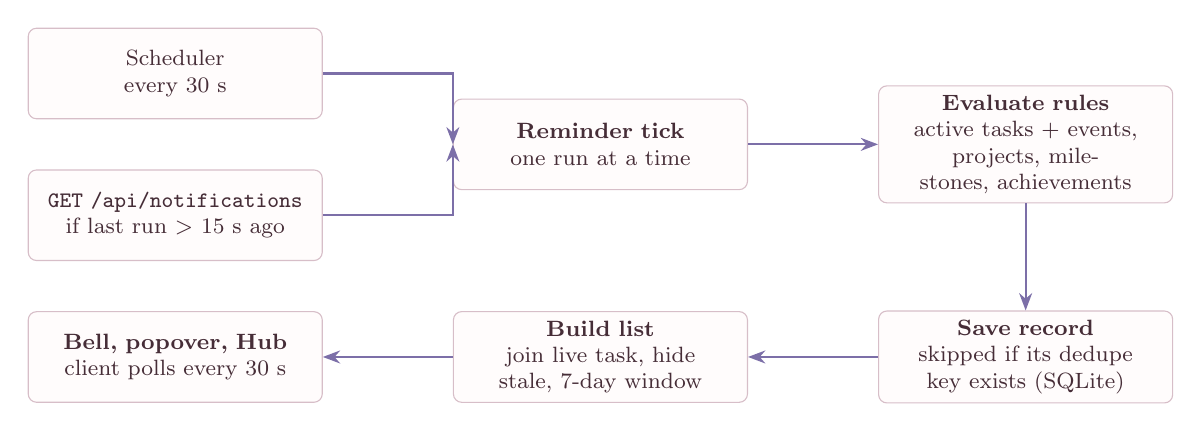
\begin{tikzpicture}[
  box/.style={draw=edge, fill=card, rounded corners=3pt, text width=3.5cm, align=center, minimum height=1.15cm, font=\footnotesize, text=ink},
  arr/.style={-{Stealth[length=2.2mm]}, thick, draw=accent},
  lab/.style={font=\scriptsize, text=muted, align=center}]
  \node[box] (tick) at (0.3,0.9) {Scheduler\\ every 30 s};
  \node[box] (get) at (0.3,-0.9) {\texttt{GET /api/notifications}\\ if last run $>$ 15 s ago};
  \node[box] (run) at (5.7,0) {\textbf{Reminder tick}\\ one run at a time};
  \node[box] (eval) at (11.1,0) {\textbf{Evaluate rules}\\ active tasks + events, projects, milestones, achievements};
  \node[box] (save) at (11.1,-2.7) {\textbf{Save record}\\ skipped if its dedupe key exists (SQLite)};
  \node[box] (list) at (5.7,-2.7) {\textbf{Build list}\\ join live task, hide stale, 7-day window};
  \node[box] (ui) at (0.3,-2.7) {\textbf{Bell, popover, Hub}\\ client polls every 30 s};
  \draw[arr] (tick.east) -- (run.west |- tick.east) -- (run.north west |- tick.east) -- (run.west);
  \draw[arr] (get.east) -- (run.west |- get.east) -- (run.south west |- get.east) -- (run.west);
  \draw[arr] (run) -- (eval);
  \draw[arr] (eval) -- (save);
  \draw[arr] (save) -- (list);
  \draw[arr] (list) -- (ui);
\end{tikzpicture}
\caption{Notification pipeline. The scheduler and the list request both start the same tick, so alerts still appear if the timer was paused.}
\end{hfig}

\subsection{What notifies, and when}

\begin{longtable}{@{}p{2.3cm}p{3.6cm}p{4.2cm}p{4.4cm}@{}}
\toprule
\textbf{Source} & \textbf{Due soon} & \textbf{Overdue} & \textbf{Opens} \\
\midrule
\endhead
Task (active) & At its reminder time (Figure~\ref{fig:timeline}) & When the deadline has passed & \texttt{/tasks/hub?task=<id>} \\
Event & Start is within 24 h & Start has passed & \texttt{/events?item=<id>} \\
Project & Deadline within 24 h & Deadline has passed & \texttt{/focus?item=<id>} \\
Milestone & Target date within 24 h & Target date has passed & \texttt{/milestones?item=<id>} \\
Achievement & Future date within 24 h, reminder switched on & Date has passed & \texttt{/achievements?item=<id>} \\
\bottomrule
\end{longtable}

Exclusions: class events and canceled events; finished or paused projects; achieved milestones; completed tasks. A date without a time counts as 23:59 of that day. A source more than 24 h away does not notify.

\subsection{Task reminder timing}

\begin{hfig}
\centering
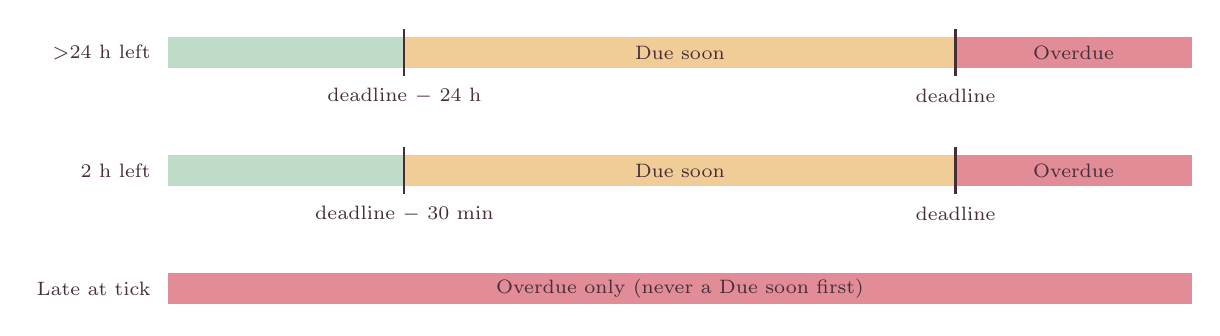
\begin{tikzpicture}[lab/.style={font=\scriptsize, text=ink}, tk/.style={thick, draw=ink}]
  % Row 1: created with more than 24 h left
  \node[lab, anchor=east] at (-0.1,2.4) {$>$24 h left};
  \fill[sage] (0,2.2) rectangle (3.0,2.6);
  \fill[amber] (3.0,2.2) rectangle (10.0,2.6);
  \fill[rose] (10.0,2.2) rectangle (13.0,2.6);
  \draw[tk] (3.0,2.1) -- (3.0,2.7);
  \draw[tk] (10.0,2.1) -- (10.0,2.7);
  \node[lab] at (3.0,1.85) {deadline $-$ 24 h};
  \node[lab] at (10.0,1.85) {deadline};
  \node[lab] at (6.5,2.4) {Due soon};
  \node[lab] at (11.5,2.4) {Overdue};
  % Row 2: created with 2 h left
  \node[lab, anchor=east] at (-0.1,0.9) {2 h left};
  \fill[sage] (0,0.7) rectangle (3.0,1.1);
  \fill[amber] (3.0,0.7) rectangle (10.0,1.1);
  \fill[rose] (10.0,0.7) rectangle (13.0,1.1);
  \draw[tk] (3.0,0.6) -- (3.0,1.2);
  \draw[tk] (10.0,0.6) -- (10.0,1.2);
  \node[lab] at (3.0,0.35) {deadline $-$ 30 min};
  \node[lab] at (10.0,0.35) {deadline};
  \node[lab] at (6.5,0.9) {Due soon};
  \node[lab] at (11.5,0.9) {Overdue};
  % Row 3: already overdue
  \node[lab, anchor=east] at (-0.1,-0.6) {Late at tick};
  \fill[rose] (0,-0.8) rectangle (13.0,-0.4);
  \node[lab] at (6.5,-0.6) {Overdue only (never a Due soon first)};
\end{tikzpicture}
\caption{Alert timeline. Rule: 24 h or more left gives deadline $-$ 24 h; less than 24 h gives deadline $-$ (remaining $\div$ 4). Row 1 and 2 are not drawn to one scale.}\label{fig:timeline}
\end{hfig}

\subsection{What clears or removes a notification}

\begin{tabular}{@{}p{5.2cm}p{10.9cm}@{}}
\toprule
\textbf{Action} & \textbf{Effect} \\
\midrule
Complete a task & Deletes its Due soon / Overdue alerts. \textbf{New in v4.2:} creates nothing. \\
Reopen a task & Deletes any leftover Completed row; the reminder is recomputed. \\
Change a task's deadline, or transfer it & Deletes its Due soon / Overdue alerts; a new alert can follow the new deadline. \\
Delete a task & Deletes all its notifications. \\
Change an event, project or milestone date & Old alert is hidden because the stored deadline no longer matches the source. \\
Retention & Anything older than 7 days is purged (hourly) and never listed. \\
Mark read / unread / mark all & Sets or clears the read time. Opening the linked item marks it read. \\
\bottomrule
\end{tabular}

A dedupe key (task id or source key, kind, deadline) guarantees one alert per item, kind and deadline, even if the tick runs many times.

\subsection{Observations}

\begin{enumerate}
  \item A task can show both \emph{Due soon} and \emph{Overdue} entries, as in your screenshot. This is by design: each is a separate alert.
  \item The older \emph{Due soon} card in the screenshot shows ``Overdue by 8m''. The title is frozen at creation, but the time-left line is computed live. After the deadline the two lines contradict each other.
  \item The Hub still lists a \emph{Completed} filter chip. It will now always read 0.
\end{enumerate}

\newpage
\section{Read versus unread: proposals}\label{sec:proposals}

\textbf{Why it is hard to read today.} Unread is a 6\% accent tint on the card, a 8 px dot and an empty checkbox. Read is a white card with a ticked box. The tint is close to invisible on a pale pink theme, titles have the same weight in both states, and a ticked box reads as ``active'' when it means ``done''.

\begin{hfig}
\centering
\newcommand{\ctl}[3]{% x y kind
  \ifcase#3
    \draw[ink, rounded corners=1.5pt, thick] (#1-0.13,#2-0.13) rectangle (#1+0.13,#2+0.13);
  \or
    \draw[accent, fill=accent, rounded corners=1.5pt] (#1-0.13,#2-0.13) rectangle (#1+0.13,#2+0.13);
    \draw[white, thick] (#1-0.07,#2) -- (#1-0.02,#2-0.07) -- (#1+0.08,#2+0.07);
  \or
    \fill[accent] (#1,#2) circle (0.13);
  \or
    \draw[muted, thick] (#1,#2) circle (0.13);
  \fi}
\newcommand{\ncard}[9]{% x y fill bar titlefont titlecolor kind tag age
  \draw[edge, fill=#3, rounded corners=3pt] (#1,#2) rectangle ++(7.4,-1.55);
  \ifx\relax#4\else\fill[#4] (#1+0.02,#2-0.04) rectangle ++(0.1,-1.47);\fi
  \node[anchor=west, font=\scriptsize, fill=white, draw=edge, rounded corners=5pt, inner sep=2pt, text=ink] at (#1+0.35,#2-0.3) {#8};
  \node[anchor=west, font=\footnotesize, text=#6] at (#1+0.35,#2-0.75) {#5 Notice title};
  \node[anchor=west, font=\scriptsize, text=muted] at (#1+0.35,#2-1.2) {#9};
  \ctl{#1+7.0}{#2-0.3}{#7}}
\begin{tikzpicture}
  \node[font=\small\bfseries] at (3.7,0.45) {Today};
  \node[font=\small\bfseries] at (11.7,0.45) {Proposal A + B (recommended)};
  % Today
  \ncard{0}{0}{white}{\relax}{\bfseries}{ink}{1}{Overdue}{7 min ago}
  \ncard{0}{-1.8}{tint}{\relax}{\bfseries}{ink}{0}{Due soon}{42 min ago}
  \fill[rose] (0.2,-2.55) circle (0.06);
  % Proposal
  \ncard{8}{0}{gray!8}{\relax}{\mdseries}{muted}{3}{Overdue}{7 min ago}
  \ncard{8}{-1.8}{white}{accent}{\bfseries}{ink}{2}{Due soon}{42 min ago}
  \node[font=\scriptsize, text=muted] at (3.7,-3.7) {tint only, dot beside title};
  \node[font=\scriptsize, text=muted] at (11.7,-3.7) {bar, bold, filled dot  vs  dimmed, plain, hollow};
\end{tikzpicture}
\caption{Left: current cards (top read, bottom unread). Right: unread has a left accent bar, bold title and a filled dot as the control; read is dimmed with regular weight and a hollow dot.}
\end{hfig}

\begin{longtable}{@{}p{0.7cm}p{4.6cm}p{6.0cm}p{4.3cm}@{}}
\toprule
 & \textbf{Idea} & \textbf{Effect} & \textbf{Cost / risk} \\
\midrule
\endhead
A & \textbf{Accent bar and weight.} Unread: 4 px left bar, semibold title, full-ink message. Read: dimmed, regular weight, no bar. & Visible in a glance at any zoom; works without colour (weight and bar). & Small change to one component. \\
B & \textbf{Dot as the control.} Replace the checkbox with one filled-or-hollow dot button (mail-app convention). Same click target, same aria labels. & Fixes the ``ticked means done'' confusion; one symbol instead of dot plus box. & Hub and popover tests reference the checkbox. \\
C & \textbf{New / Earlier sections.} Sticky ``New (n)'' group above ``Earlier''. & Unread items are always on top and counted. & Reorders the list; Hub already groups by date, so the two groupings need a rule. \\
D & \textbf{Compact read rows.} Read items collapse to one line (tag, title, age); unread keep the full card. & Unread cards dominate; the panel shows more items. & Message of read items hidden; changes the 14-item footer layout. \\
E & \textbf{Unread filter in popover.} A segmented ``All / Unread'' switch like the Hub. & Fast triage when many items. & Extra control in a small panel; does not fix the card itself. \\
\bottomrule
\end{longtable}

\begin{hfig}
\centering
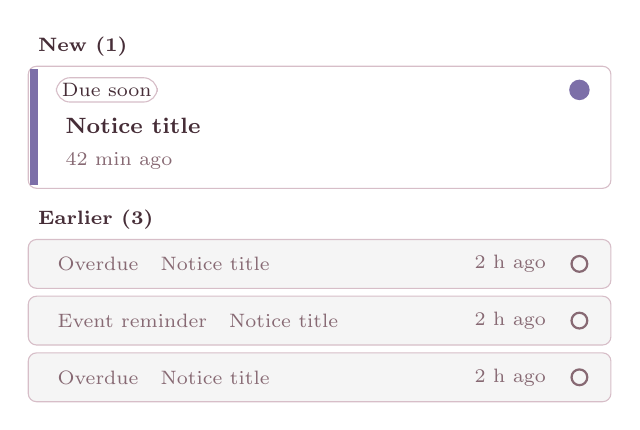
\begin{tikzpicture}
  \node[anchor=west, font=\scriptsize\bfseries, text=ink] at (0,0.25) {New (1)};
  \draw[edge, fill=white, rounded corners=3pt] (0,0) rectangle ++(7.4,-1.55);
  \fill[accent] (0.02,-0.04) rectangle ++(0.1,-1.47);
  \node[anchor=west, font=\scriptsize, fill=white, draw=edge, rounded corners=5pt, inner sep=2pt, text=ink] at (0.35,-0.3) {Due soon};
  \node[anchor=west, font=\footnotesize\bfseries, text=ink] at (0.35,-0.75) {Notice title};
  \node[anchor=west, font=\scriptsize, text=muted] at (0.35,-1.2) {42 min ago};
  \fill[accent] (7.0,-0.3) circle (0.13);
  \node[anchor=west, font=\scriptsize\bfseries, text=ink] at (0,-1.95) {Earlier (3)};
  \foreach \i/\t in {0/Overdue,1/Event reminder,2/Overdue} {
    \draw[edge, fill=gray!8, rounded corners=3pt] (0,{-2.2-\i*0.72}) rectangle ++(7.4,-0.62);
    \node[anchor=west, font=\scriptsize, text=muted] at (0.25,{-2.51-\i*0.72}) {\t \quad Notice title};
    \node[anchor=east, font=\scriptsize, text=muted] at (6.7,{-2.51-\i*0.72}) {2 h ago};
    \draw[muted, thick] (7.0,{-2.51-\i*0.72}) circle (0.1);
  }
\end{tikzpicture}
\caption{Options C and D together: unread card on top, read items as compact rows under ``Earlier''.}
\end{hfig}

\textbf{Recommendation.} Ship \textbf{A + B} first: they change one component, fix both the visibility and the checkbox meaning, and keep the layout the same. Add \textbf{E} later only if the panel regularly holds many items. Leave \textbf{C} and \textbf{D} for a separate decision because they change list structure.

\textbf{Decisions for you.}
\begin{enumerate}
  \item Which options to build (recommended: A + B).
  \item Remove the Hub's \emph{Completed} chip now that it is always 0?
  \item Stop showing an older \emph{Due soon} card once the same item has an \emph{Overdue} one, to remove the contradictory line in the screenshot?
\end{enumerate}

\section{Verification}

Changed files: \texttt{src/services/task-service.ts}, \texttt{src/services/notification-service.ts}, and the two matching service tests. The task and notification service tests pass (73 of 74 tests across the services folder and the notification filter). The one failing test, in \texttt{tests/services/event-draft-service.test.ts}, stops on ``Legacy JSON data exists outside DATA\_DIR'' and does not touch this change. A full type check reports errors only in \texttt{tests/features/projects/projects-view.test.tsx}, which is outside this work.

\end{document}



